% !TeX document-id = {ed9f9aeb-6fc7-4042-9422-9ce343a26700}
\documentclass[12pt]{article}

\usepackage{multirow}
\usepackage{multicol}
\usepackage{framed}
%\usepackage{mdframed}
\usepackage{setspace}
\usepackage{color}
\usepackage{xcolor}
\usepackage{hyperref}
\usepackage[pdftex]{graphicx}
\usepackage{keystroke}
\usepackage{lipsum} 
\usepackage[utf8]{inputenc}
\usepackage[english]{babel}
\usepackage{textcomp}
\usepackage[T1]{fontenc} 
\usepackage{MnSymbol,wasysym}
\usepackage{tikzsymbols}

\usepackage{enumitem}
\setlist[description]{leftmargin=\parindent,labelindent=\parindent}

\usepackage{geometry}
 \geometry{
 left=20mm,
 right=10mm,
 top=20mm,
 }

\textwidth=7.0in
\topmargin=-0.6in
\leftmargin=0.5in
\textheight=9.25in
\hoffset=-0.5in
\footskip=0.2in

%\usepackage{pygmentize}
\usepackage{minted}
%\newminted[python]{python}{frame=single}
%\fvset{showspaces}
%\renewcommand\FancyVerbSpace{\textcolor{mygray}{\char32}}
\setminted[text]{
	escapeinside=||, 
	%breaksymbolleft=\carriagereturn,
	frame=single,
	%showspaces=true
	framesep=2mm,
	baselinestretch=1.2,
	bgcolor=mygray
}

% all 4 borders
%\newmdenv{allfour}

\hypersetup{
    %bookmarks=true,         % show bookmarks bar?
    unicode=false,          % non-Latin characters in Acrobat’s bookmarks
    pdftoolbar=true,        % show Acrobat’s toolbar?
    pdfmenubar=true,        % show Acrobat’s menu?
    pdffitwindow=false,     % window fit to page when opened
    pdfstartview={FitH},    % fits the width of the page to the window
    pdftitle={My title},    % title
    pdfauthor={Author},     % author
    pdfsubject={Subject},   % subject of the document
    pdfcreator={Creator},   % creator of the document
    pdfproducer={Producer}, % producer of the document
    pdfkeywords={keyword1, key2, key3}, % list of keywords
    pdfnewwindow=true,      % links in new PDF window
    colorlinks=true,       % false: boxed links; true: colored links
    linkcolor=red,          % color of internal links (change box color with linkbordercolor)
    citecolor=green,        % color of links to bibliography
    filecolor=magenta,      % color of file links
    urlcolor=blue           % color of external links
}

%\mdfsetup{
%  linewidth=.5bp,
%  innerleftmargin=3.5bp,
%  innerrightmargin=3.5bp,
%  innertopmargin=.5bp,
%  innerbottommargin=.5bp,
%}

% windows logo
% Lower the picture a little to match the text baseline
\newcommand{\WindowsLogo}{\raisebox{-0.1em}{%
  
\includegraphics[height=0.8em]{win_logo}}}
\newcommand{\WinKey}{\keystroke{\WindowsLogo}}

\newcommand{\CTRL}{\raisebox{-0.1em}{Ctrl}}
\newcommand{\CTRLKey}{\keystroke{\CTRL}}

\newcommand{\ALT}{\raisebox{-0.1em}{Alt}}
\newcommand{\ALTKey}{\keystroke{\ALT}}

\newcommand{\ENTER}{\raisebox{-0.1em}{Enter}}
\newcommand{\ENTERKey}{\keystroke{\ENTER}}

%\pagestyle{myheadings}
%\markright{{\large ME 4140 Fall 2019---The Robotic Operating System}}

\definecolor{monokaibg}{HTML}{272822}
\definecolor{friendlybg}{HTML}{f0f0f0}
\definecolor{mygreen}{rgb}{0.1333 ,  0.5451,    0.1333}
\definecolor{mypink}{rgb}{0.1333 ,  0.5451,    0.1333}
\definecolor{mygreen}{rgb}{0, .39, 0}
%\definecolor{dred}{#8B0000} 
\definecolor{mypurple}{rgb}{0.6,0.1961,0.8}
\definecolor{mybrown}{rgb}{0.5451,0.2706,0.0745}
\definecolor{mygray}{rgb}{.83, .83, .83}

\newcommand{\R}{\color{red}}
\newcommand{\B}{\color{blue}}
\newcommand{\K}{\color{black}}
%\newcommand{\G}{\color{mygreen}}
\newcommand{\PR}{\color{mypurple}}
\newcommand{\GY}{\color{mygray}}

\newcommand{\VA}{\vspace{2mm}}
\newcommand{\VB}{\vspace{5mm}} 
\newcommand{\VC}{\vspace{30mm}} 

\newcommand{\SQ}{\textquotesingle} 

\begin{document}

%\thispagestyle{plain}

%\thispagestyle{plain}

\begin{center}
   {\bf \Large ROS Workshop - Tutorial 2 - Installing ROS}\vspace{3mm} \\
   {\bf \large ME 4140 - Introduction to Robotics - Fall 2020} \vspace{5mm}\\
\end{center}

\begin{description}

\item[\textbf{\underline{Overview:}}] \hfill \vspace{3mm}\\
After completing {\it Tutorial 1 - Virtualize Ubuntu}, your new operating system is running, and you are ready to install ROS. You can read more about this installation \href{http://wiki.ros.org/melodic/Installation/Ubuntu}{here} on the wiki.

\item[\textbf{\underline{System Requirements:}}] \hfill \vspace{0mm}

\begin{itemize}
	\item {\bf OS}: This tutorial is inteded for the Ubuntu 18.04 LTS operating system. Alternate flavors of 18.04 (i.e. - Mint, Mate, kbuntu) may work but have not been tested.
	\item {\bf Internet:} Your computer must be connected to the internet to proceed. Downloading and installing ROS may take approximately 15 to 30 minutes .


\end{itemize}

\item[\textbf{\underline{Disclaimer:}}] \hfill \vspace{0mm}

\begin{itemize}
	\item {\bf\R Copy and Paste Errors:} {\R It is strongly recommended to download this PDF and view it in Ubuntu so that you can copy and paste the required commands correctly.}

	\item {\bf Backup: } If you are using a virtual machine, it is recommend to make a snaphot of your virtual machine in case you want to revert. See {\it Tutorial 1 - Virtualize Ubuntu } for details.   
\end{itemize}

\item[\textbf{\underline{Installation Instructions:}}] \hfill \vspace{0mm}

You will enter several commands into the terminal during this tutorial. { \bf The terminal commands are shown in gray boxes.} Press \CTRLKey+\ALTKey+{\bf T} to open a new terminal, then carefully copy each command and paste it into the terminal then press \ENTERKey.


\begin{enumerate}
	
	
	\item  Setup your sources.list to accept software from packages.ros.org.

	\begin{minted}{text}
sudo sh -c 'echo "deb http://packages.ros.org/ros/ubuntu \
|\$|(lsb_release -sc) main" > /etc/apt/sources.list.d/ros-latest.list'
	\end{minted}
	
	\item Set up your keys which are used authenitcate software packages for security.
	
	\begin{minted}[]{text}
sudo apt-key adv --keyserver 'hkp://keyserver.ubuntu.com:80'\
--recv-key C1CF6E31E6BADE8868B172B4F42ED6FBAB17C654	
	\end{minted}
				
	\item Update your Ubuntu system. It is a good idea to do this daily.  
	
	\begin{minted}[]{text}
sudo apt update
	\end{minted}

\newpage
	
	\item Download and install ROS Melodic Desktop-Full. Depending on your network connection this step will take some time. Now is a good time to get a \Coffeecup \Cooley.  
	
	\begin{minted}[]{text}
sudo apt install ros-melodic-desktop-full
	\end{minted}


	\item Initialize rosdep (2 separate commands) 
	\begin{minted}[]{text}
sudo rosdep init
	\end{minted}
	
	\begin{minted}[]{text} 
rosdep update
	\end{minted}

\item Evironment Setup (2 separate commands) 
\begin{minted}{text} 
echo "source /opt/ros/melodic/setup.bash" >> ~/.bashrc
\end{minted}

\begin{minted}{text} 
source ~/.bashrc 
\end{minted}
		
\item Install Development Tools. You are almost there! 
\begin{minted}{text} 
sudo apt install python-rosinstall python-rosinstall-generator \ 
python-wstool build-essential
\end{minted}

After completing Step 7 you have installed ROS on your Ubuntu system. Now it is time to test the installation. 
\end{enumerate}

\newpage

\item[\textbf{\underline{Test ROS Installation}}]

\item Close all open terminal windows. Next, open a new terminal and try the following command.\\
\begin{minted}{text}  
roscore
\end{minted}

If the installation was successful, the terminal output will be {\it similar} to the image below. \vspace{3mm}\\

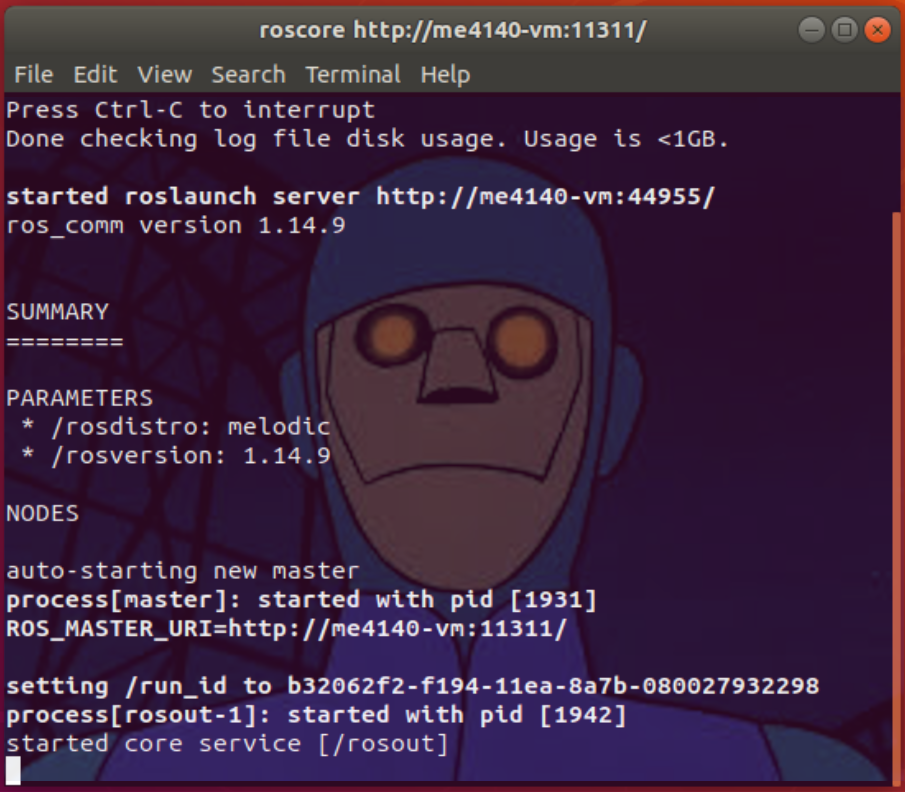
\includegraphics[scale=1]{roscore_charlie.png}

		%\item If you see ROS start in the terminal your ROS installation was successful!


\end{description}
\end{document}
